\documentclass[10pt,twocolumn]{article}

\usepackage[utf8]{inputenc}
\usepackage{setspace}
\usepackage[letterpaper,margin=1.5cm]{geometry}
\usepackage{pgfplots}
\usepackage{pgfplotstable}
\pgfplotsset{compat=newest}
\usetikzlibrary{shapes,backgrounds}
\usepgfplotslibrary{ternary}
\usepgfplotslibrary{external} 
%\tikzexternalize

\author{Timoth\'ee Poisot \and Philippe Desjardins-Proulx \and Dominique Gravel}
\title{A phenomenological model of metacommunity coevolution}
\usepackage{microtype}
\usepackage[loosequotes,lf]{MinionPro}
\usepackage{biblatex}
\usepackage{graphicx}
\bibliography{library}

%% Tikz styles
\tikzstyle{sp} = [circle, text width=1.5cm, inner sep = 0pt]
\tikzstyle{pop} = [diamond, text width=0.3cm, inner sep = 0pt]

\begin{document}
	
\maketitle

\begin{abstract}
	We outline the basic ingredients for a phenomenological model of
	coevolution in spatial interaction networks. This model relies on
	developments from the insular biogeography theory and the metacommunity
	theory. We show how it can be used to derive simple predictions about the
	relative consequences of spatial structure, interaction type, and
	evolutionary pace, on the evolutionary biogeography of interactive
	metacommunities.
\end{abstract}

\section{Introduction}

Massol Ecol Lett

Despite this, \textcite{Urban2008} emphasize that the current theories leaves
us poorly prepared to handle the evolution of complex metacommunity over large
spatial extents.

\section{Ingredients of the model}

The metapopulation framework is ....

Building on these previous results, TTIB built a trophic model of island
biogeography. This model achieves the overlap between ecological network
theory and biogeography, but lacks an evolutionary component. It is the goal
of this paper to descibe how the TTIB model can be coupled to simple
evolutionary rules, to obtain a phenomenological model of evolution in
spatialized networks.

\section{Rules for evolution}

\subsection{Populations and species delineation}

Our model assumes that each population $i$ occupies a position
$\mathbf{n}_{i}$ in the hyperdimensional niche space. Given the position of
all its populations, the center of mass of a species can be taken by averaging
the position of each population allong each niche axis. This center of mass,
for species $s$, is called $\mathbf{m}_s$. Everytime a species colonizes a new
patch, it creates a new population in the model.

\begin{figure}[tb]
	\centering
	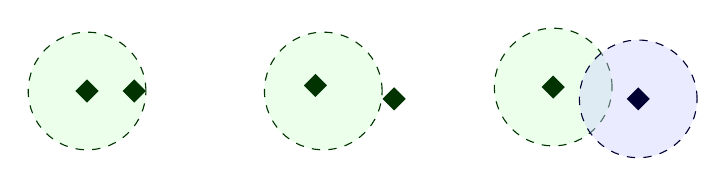
\begin{tikzpicture}

	\node[sp, fill opacity = 0.4, style = dashed, fill = green!20, draw = green!20!black] at (0, 0) {};
	\node[pop, fill=green!20!black] (s1p1) at (0,0) {};
	\node[pop, fill=green!20!black] (s1p1) at (0.6,0) {};

	\node[sp, fill opacity = 0.4, style = dashed, fill = green!20, draw = green!20!black] at (3, 0) {};
	\node[pop, fill=green!20!black] (s1p1) at (2.9,0.07) {};
	\node[pop, fill=green!20!black] (s1p1) at (3.9,-0.1) {};	

	\node[sp, fill opacity = 0.4, style = dashed, fill = green!20, draw = green!20!black] at (5.92, 0.05) {};
	\node[pop, fill=green!20!black] (s1p1) at (5.92,0.05) {};
	\node[sp, fill opacity = 0.4, style = dashed, fill = blue!20, draw = blue!20!black] (s1p1) at (7.0,-0.1) {};	
	\node[pop, fill=blue!20!black] (s1p1) at (7.0,-0.1) {};

\end{tikzpicture}
	\caption{Conceptual model of speciation. Each species is defined by the
	center of mass of all its populations on the niche space, and a fixed
	distance. When one population falls outside of this distance, as in the
	case in the second step, it forms a new species. Note that, as the
	position of each population on the niche space changes randomly to
	simulate the effect of drift, the center of mass of the species will move
	through time.}
   \label{f:speciation}
\end{figure}

\subsection{Speciation}

The model assumes a fixed treshold $\sigma$, for which every population whose
$\mathrm{d}\left(\mathbf{m}_s,\mathbf{n}_i\right) \geq \sigma$, where
$\mathrm{d}$ is any distance function, undergoes speciation. This process is
illustrated in Fig.~\ref{f:speciation}. As the center of mass of each species,
and consequently the criteria for speciation, is calculated at the regional
scale, our model does not allow sympatric speciation.

\subsection{Genetic drift}

\section{Rules for interaction}

The existence of an interaction follows the same rules as in the niche model
of  \textcite{Williams2000}. Each population is identified by its position $n$ on
a niche space, which can be composed of as many arbitrary continuous
quantitative niche axes as needed. On each axis, each population has a centroïd
$c$, and a range $r$, meaning that each species will interact with any other
species whose trait value falls within $n+c\pm r$. This relationship holds for
each axis of the niche space, meaning that, for a $k$ dimensional niche space,
a species $i$ is represented by the arrays $\mathbf{n}_i=\{n_{i1}, n_{i2},
..., n_{ik}\}$, $\mathbf{c}_i=\{c_{i1}, c_{i2}, ..., c_{ik}\}$, and
$\mathbf{r}_i=\{r_{i1}, r_{i2}, ..., r_{ik}\}$.

We assume that, for two populations $i$ and $j$ to interact, their niche
positions need to be compatible on all axes. This allows an adjancency matrix
of all potential interactions among existing populations to be calculated by

\begin{equation}\label{e:potential}
	\mathbf{A}_{ij} = \prod_{a=0}^k \delta\left(n_{ia}+r_{ia}-c_{ia} \leq n_{ja} \leq n_{ia}+r_{ia}+c_{ia} \right)
\end{equation}

\noindent , in which $\delta$ is Kronecker's delta function, taking a value of
one when the condition is satisfied, and zero otherwise. This formulation
lends itself nicely to simplifications. Intra-specific interactions can be
easily forbiden. In addition, if one designs two or more sets of species (so
as to simulate bipartite or tripartite networks), and fixes as a an
evolutionary rule that speciation can never switch a population from one set
to the other (a reasonnable assumption over micro-evolutionary times), all
within-set interactions can be set to zero. A general expression of the
metaweb adjacency matrix is therefore given by

\begin{equation}\label{e:realized}
	\mathbf{M}_{ij} = \delta_{\mathrm{sp}}\times\delta_{\mathrm{set}}\times\mathbf{A}_{ij}
\end{equation}

\noindent , in which $\delta_\mathrm{sp}$ is the existence of intra-specific
interactions, and $\delta_\mathrm{set}$ is the existence of intra-set
interactions.

\begin{figure}[tb]
	\centering
	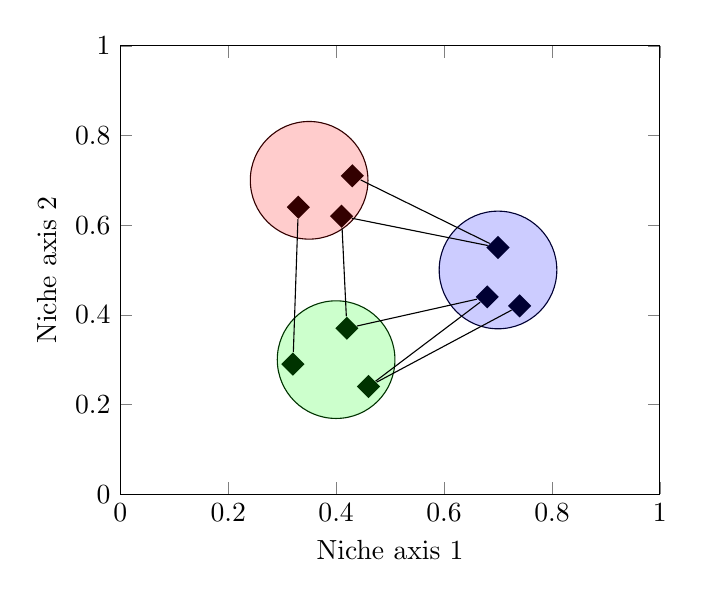
\begin{tikzpicture}
	\begin{axis}[
		xlabel={Niche axis 1},
		ylabel={Niche axis 2},
		xmin = 0, xmax = 1,
		ymin = 0, ymax = 1,
		enlargelimits = 0
		]
		%%% Species circles
		\node[sp, fill=green!20, draw=green!20!black] at (axis cs:0.4,0.3) {};
		\node[sp, fill=blue!20,draw=blue!20!black] at (axis cs:0.7,0.5) {};
		\node[sp, fill=red!20,draw=red!20!black] at (axis cs:0.35,0.7) {};
		
		%%% Populations
		\node[pop, fill=green!20!black] (s1p1) at (axis cs:0.42,0.37) {};
		\node[pop, fill=green!20!black] (s1p2) at (axis cs:0.32,0.29) {};
		\node[pop, fill=green!20!black] (s1p3) at (axis cs:0.46,0.24) {};

		\node[pop, fill=blue!20!black] (s2p1) at (axis cs:0.68,0.44) {};
		\node[pop, fill=blue!20!black] (s2p2) at (axis cs:0.74,0.42) {};
		\node[pop, fill=blue!20!black] (s2p3) at (axis cs:0.70,0.55) {};

		\node[pop, fill=red!20!black] (s3p1) at (axis cs:0.33,0.64) {};
		\node[pop, fill=red!20!black] (s3p2) at (axis cs:0.41,0.62) {};
		\node[pop, fill=red!20!black] (s3p3) at (axis cs:0.43,0.71) {};

		%%% Interactions
		\draw [-] (s3p1) to (s1p2);
		\draw [-] (s3p2) to (s1p1);
		\draw [-] (s1p3) to (s2p1);
		\draw [-] (s1p1) to (s2p1);
		\draw [-] (s1p3) to (s2p2);
		\draw [-] (s3p3) to (s2p3);
		\draw [-] (s3p2) to (s2p3);
	\end{axis}
\end{tikzpicture}
	\caption{Example of three species, each made of several populations, on a
	two-axes niche represented in the unit square. Each circle correspond to
	the limits of one species, and each diamond on the niche space is a
	population. Populations which are close enough are connected. }
   \label{f:interactions}
\end{figure}

Note that because different populations are representing each species locally,
there will be a turnover in the existence of interactions at the species
level, which is a realistic feature of natural interacting metacommunities
\parencite{PoisotELE2012}. Two species are interacting if they have at least
one interaction between their populations.

\section{Metacommunity dynamics}

\section{Conclusion}

\printbibliography

\end{document}